\documentclass[aspectratio=169]{beamer}

\usepackage{amsmath, amssymb}
\usepackage{tikz}
\usepackage{booktabs}
\usepackage{xcolor}
\usepackage{graphicx}
\usepackage{colortbl}

\usetikzlibrary{arrows.meta, positioning, calc, shapes.geometric}

\usefonttheme{professionalfonts}
\setbeamertemplate{navigation symbols}{}

% --- Color theme (white/professional) ---
\definecolor{darktext}{HTML}{1A1A2E}
\definecolor{accent}{HTML}{2D3494}
\definecolor{accentblue}{HTML}{1565C0}
\definecolor{accentgreen}{HTML}{2E7D32}
\definecolor{accentred}{HTML}{C62828}
\definecolor{accentorange}{HTML}{E65100}
\definecolor{accentteal}{HTML}{00695C}
\definecolor{midgray}{HTML}{555555}
\definecolor{lightgray}{HTML}{999999}
\definecolor{boxfill}{HTML}{F0F2F8}
\definecolor{boxfillgreen}{HTML}{EDF7ED}
\definecolor{boxfillred}{HTML}{FDECEC}
\definecolor{boxfillorange}{HTML}{FFF3E0}
\definecolor{boxfillblue}{HTML}{E8EAF6}

\setbeamercolor{background canvas}{bg=white}
\setbeamercolor{normal text}{fg=darktext}
\setbeamercolor{frametitle}{fg=accent}
\setbeamercolor{itemize item}{fg=accent}
\setbeamercolor{itemize subitem}{fg=accentblue}

\setbeamertemplate{itemize item}{\textbullet}
\setbeamertemplate{itemize subitem}{--}

\setbeamersize{text margin left=8mm, text margin right=8mm}

% --- page number ---
\setbeamertemplate{footline}{%
    \raisebox{8pt}{\makebox[\paperwidth]{\hfill\makebox[6em]{\color{lightgray}\small\texttt{\insertframenumber/\inserttotalframenumber}}}}%
}

% --- Custom commands ---
\newcommand{\accentline}{\vspace{1pt}{\color{accent}\rule{0.3\textwidth}{1.5pt}}\vspace{4pt}}
\newcommand{\resultbox}[3][boxfill]{%
    \begin{tikzpicture}
    \node[fill=#1, rounded corners=3pt, draw=#2, line width=0.8pt, text width=\linewidth-16pt, inner sep=6pt, text=darktext] {#3};
    \end{tikzpicture}%
}

\title{}
\author{}
\date{}

\begin{document}

% ============================================================
% SLIDE 1: Title
% ============================================================
\begin{frame}[plain]
    \vspace{1.8cm}
    \begin{center}
        {\color{accent}\rule{0.5\textwidth}{1.5pt}}\\[10pt]
        {\LARGE\bfseries\color{darktext} Lobbying, Corruption, and Contagion\\[4pt] on Council Networks}\\[10pt]
        {\large\color{accentblue} Literature Review}\\[20pt]
        {\color{midgray} Samir Kadariya \& Bryce Roberts}\\[4pt]
        {\small\color{lightgray} 14.18xt }
    \end{center}
\end{frame}

% ============================================================
% SLIDE 2: Motivation & Overview
% ============================================================
\begin{frame}{Motivation}
\accentline
\begin{columns}[T]
    \begin{column}{0.48\textwidth}
        {\color{accent}\bfseries Our Research Question}\\[4pt]
        {\small A lobbyist seeks to pass legislation through a council whose members are connected by social and political ties. In this sort of scneario, we wanted to look into:}
        \begin{itemize}\small
            \item Whom should the lobbyist target with bribes?
            \item How does corruption spread through the network?
            \item What institutional designs resist outside influence?
        \end{itemize}
    \end{column}
    \begin{column}{0.48\textwidth}
        {\color{accent}\bfseries Papers}\\[4pt]
        \begin{enumerate}\small
            \item {\color{accentred}\bfseries Shleifer \& Vishny (1993)} --- The economics of corruption
            \item {\color{accentgreen}\bfseries Galeotti, Golub, \& Goyal (2020)} --- Optimal targeting on networks
            \item {\color{accentteal}\bfseries Morris (2000)} --- Contagion on networks
        \end{enumerate}
        \vspace{6pt}
        {\small\color{midgray} Together these address: the mechanics of bribery, whom to target in a network, and when behavior spreads contagiously.}
    \end{column}
\end{columns}
\end{frame}

% ============================================================
% SLIDE 3: Shleifer & Vishny — Setup
% ============================================================
\begin{frame}[shrink=5]{Shleifer \& Vishny (1993) --- ``Corruption''}
\accentline
\begin{columns}[T]
    \begin{column}{0.50\textwidth}
        {\color{accentred}\bfseries Core Idea}\\[3pt]
        {\small Government officials act as \textbf{monopolists} selling government goods (permits, licenses) and extract bribes.}\\[6pt]

        {\color{accentred}\bfseries Model}\\[2pt]
        \begin{itemize}\small\setlength\itemsep{2pt}
            \item Good with demand $D(p)$, official price $p$
            \item Official restricts supply to extract bribes
            \item \textbf{Without theft:} total price $= p + \text{bribe}$
            \item \textbf{With theft:} official hides sale; price $\leq p$
        \end{itemize}

        \vspace{4pt}
        {\color{accentred}\bfseries Example}\\[2pt]
        {\small A builder needs permits from fire, water, and zoning agencies. Each independently charges a bribe, ignoring the effect on the others.}
    \end{column}
    \begin{column}{0.46\textwidth}
        \begin{center}
        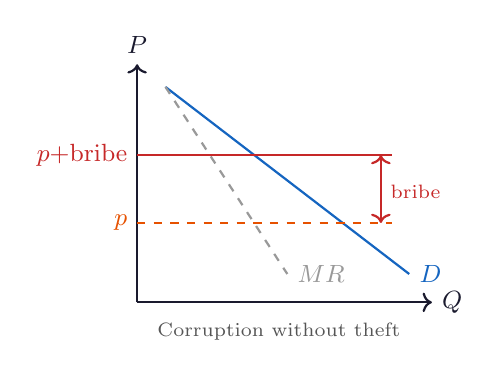
\begin{tikzpicture}[scale=0.72]
            \draw[->, thick, darktext] (0,0) -- (5.2,0) node[right] {\small $Q$};
            \draw[->, thick, darktext] (0,0) -- (0,4.2) node[above] {\small $P$};
            \draw[thick, accentblue] (0.5,3.8) -- (4.8,0.5) node[right] {\small $D$};
            \draw[thick, lightgray, dashed] (0.5,3.8) -- (2.65,0.5) node[right] {\small $MR$};
            \draw[thick, accentorange, dashed] (0,1.4) -- (4.5,1.4);
            \node[left, accentorange, font=\small] at (0,1.4) {$p$};
            \draw[thick, accentred] (0,2.6) -- (4.5,2.6);
            \node[left, accentred, font=\small] at (0,2.6) {$p{+}\text{bribe}$};
            \draw[thick, accentred, <->] (4.3,1.4) -- (4.3,2.6);
            \node[right, accentred, font=\scriptsize] at (4.3,1.95) {bribe};
            \node[below, midgray, font=\scriptsize] at (2.5,-0.2) {Corruption without theft};
        \end{tikzpicture}
        \end{center}
    \end{column}
\end{columns}
\end{frame}

% ============================================================
% SLIDE 4: Shleifer & Vishny — IO of Corruption
% ============================================================
\begin{frame}[shrink=15]{Shleifer \& Vishny --- Market Structure of Corruption}
\accentline
\begin{columns}[T]
    \begin{column}{0.55\textwidth}
        {\color{accentgreen}\bfseries 1.\ Joint Monopoly} {\small(centralized)}\\[2pt]
        {\small One entity collects all bribes, internalizes complementarities:}
        \vspace{-4pt}
        \[
            {\color{accentred} MR_1 + MR_2 \cdot \frac{dx_2}{dx_1} = MC_1}
        \]
        \vspace{-10pt}
        {\small Moderate bribes, higher output.}\\[8pt]

        {\color{accentred}\bfseries 2.\ Independent Monopolists} {\small(decentralized)}\\[2pt]
        {\small Each agency sets $MR_i = MC_i$, ignoring cross-effects.}\\
        {\small\color{accentred}\bfseries Higher per-unit bribes, lower output.}\\[8pt]

        {\color{accentteal}\bfseries 3.\ Competition}\\[2pt]
        {\small Multiple providers per good. Bribes $\to 0$.}\\[8pt]

        {\color{accentred}\bfseries Example}\\[2pt]
        {\small In post-Soviet Russia, a foreign investor must bribe the investment office, the industrial ministry, the finance ministry, and local government---each independently. Total bribe burden $\to \infty$; foreigners do not invest.}
    \end{column}
    \begin{column}{0.40\textwidth}
        \resultbox[boxfillred]{accentred}{%
            {\color{accentred}\bfseries Key Result}\\[3pt]
            {\small Decentralized corruption is \textbf{worse} than centralized---the ``tragedy of the anti-commons.''}\\[3pt]
            {\small\color{midgray} \textit{Analogy:} independent toll booths along a river. Each town ignores the effect on traffic. Total traffic collapses.}
        }
        \vspace{6pt}
        \resultbox[boxfillblue]{accent}{%
            {\color{accent}\bfseries Secrecy Cost}\\[3pt]
            {\small Corruption must be hidden $\Rightarrow$ resources shifted to bribe-friendly goods. More distortionary than taxation.}
        }
    \end{column}
\end{columns}
\end{frame}

% ============================================================
% SLIDE 5: Golub et al. — Setup
% ============================================================
\begin{frame}[shrink=5]{Galeotti, Golub, \& Goyal (2020) --- ``Targeting Interventions in Networks''}
\accentline
\begin{columns}[T]
    \begin{column}{0.60\textwidth}
        {\small $n$ agents on network $\mathbf{G}$. Each chooses action $a_i \in \mathbb{R}$. Payoff:}
        \vspace{-2pt}
        \[
            \boxed{U_i = a_i\!\left(\underbrace{b_i}_{\text{\tiny standalone}} + \underbrace{\beta \textstyle\sum_j g_{ij} a_j}_{\text{\tiny peer effects}}\right) - \underbrace{\tfrac{1}{2}a_i^2}_{\text{\tiny cost}}}
        \]
        \vspace{-6pt}
        \begin{itemize}\small\setlength\itemsep{2pt}
            \item $b_i$ = standalone marginal return (private incentive)
            \item $\beta > 0$: strategic \textbf{complements}; $\;\beta < 0$: \textbf{substitutes}
        \end{itemize}

        \vspace{4pt}
        {\color{accentgreen}\bfseries Planner's Problem}\\[2pt]
        {\small A planner with budget $C$ shifts standalone returns $\hat{b}_i \to b_i$ before the game to maximize welfare $W(\mathbf{b},\mathbf{G}) = \sum_i U_i(\mathbf{a}^*,\mathbf{G})$, subject to $\sum_i(b_i - \hat{b}_i)^2 \leq C$.}
    \end{column}
    \begin{column}{0.36\textwidth}
        \vspace{-15pt}
        \begin{center}
        {\small\color{accentgreen}\bfseries Timing}\\[1pt]
        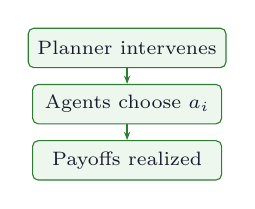
\begin{tikzpicture}[
            box/.style={fill=boxfillgreen, draw=accentgreen, rounded corners=2pt, text=darktext, font=\scriptsize, minimum width=2.4cm, minimum height=0.5cm, align=center},
            arr/.style={-{Stealth[length=3pt]}, thick, accentgreen}
        ]
            \node[box] (p) {Planner intervenes};
            \node[box, below=0.2cm of p] (a) {Agents choose $a_i$};
            \node[box, below=0.2cm of a] (w) {Payoffs realized};
            \draw[arr] (p) -- (a);
            \draw[arr] (a) -- (w);
        \end{tikzpicture}
        \end{center}

        \vspace{1pt}
        {\color{accentgreen}\bfseries Complements} {\small($\beta > 0$)}\\[1pt]
        {\small Behaviors \textbf{reinforce} each other. When a neighbor increases their action, it pushes your incentive to do the same.}\\[3pt]
        {\color{accentred}\bfseries Substitutes} {\small($\beta < 0$)}\\[1pt]
        {\small Behaviors \textbf{crowd out} each other. When a neighbor increases their action, it decreases your marginal return.}
    \end{column}
\end{columns}
\end{frame}

% ============================================================
% SLIDE 6: Golub et al. — Principal Components & Results
% ============================================================
\begin{frame}[shrink=10]{Galeotti, Golub, \& Goyal --- Main Results}
\accentline
\begin{columns}[T]
    \begin{column}{0.53\textwidth}
        {\color{accentgreen}\bfseries Eigendecomposition}\\[3pt]
        {\small Since $\mathbf{G}$ is symmetric: $\mathbf{G} = \mathbf{U}\boldsymbol{\Lambda}\mathbf{U}^\top$. In the principal component basis:}
        \[
            {\color{accentred} \underline{a}^*_\ell = \frac{1}{1 - \beta\lambda_\ell}\;\underline{b}_\ell}
        \]
        \vspace{-1pt}
        {\small The factor $\frac{1}{1-\beta\lambda_\ell}$ is the \textbf{network multiplier}---it amplifies interventions along component $\ell$.}\\[5pt]

        {\color{accentgreen}\bfseries Theorem 1}\\[2pt]
        {\small The optimal intervention's similarity to principal component $\mathbf{u}^\ell$ satisfies:}
        \[
            \rho(\mathbf{y}^*, \mathbf{u}^\ell) \;\propto\; \rho(\hat{\mathbf{b}}, \mathbf{u}^\ell)\cdot\frac{w\alpha_\ell}{\mu - w\alpha_\ell}
        \]
        \vspace{-2pt}
        {\small where $\alpha_\ell = (1{-}\beta\lambda_\ell)^{-2}$ and $\mu$ is the shadow price of the budget constraint.}
    \end{column}
    \begin{column}{0.43\textwidth}
        \resultbox[boxfillgreen]{accentgreen}{%
            {\color{accentgreen}\bfseries Complements ($\beta > 0$)}\\[3pt]
            {\footnotesize Optimal intervention targets the \textbf{first} principal component = \textbf{eigenvector centrality}.\\[2pt]
            Target the most central agents---spillovers cascade and amplify.}
        }
        \vspace{2pt}
        \resultbox[boxfillred]{accentred}{%
            {\color{accentred}\bfseries Substitutes ($\beta < 0$)}\\[3pt]
            {\footnotesize Target the \textbf{last} principal component = network bipartition. Asymmetric targeting avoids crowding out.}
        }
        \vspace{2pt}
    
    \end{column}
\end{columns}
\end{frame}

% ============================================================
% SLIDE 7: Golub et al. — Spectral Gap & Network Cohesion
% ============================================================
\begin{frame}[shrink=5]{Galeotti, Golub, \& Goyal --- The Spectral Gap}
\accentline

{\small The \textbf{spectral gap} ($\lambda_1 - \lambda_2$) determines how fast the optimal intervention becomes simple. Cohesive networks have large gaps; fragmented networks have small gaps.}

\vspace{10pt}
\begin{columns}[c]
    \begin{column}{0.45\textwidth}
        \begin{center}
        {\color{accentgreen}\bfseries\large Scenario A: High Cohesion}\\[6pt]
        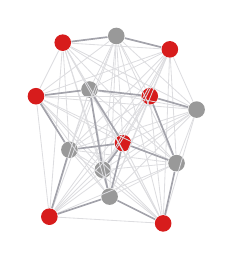
\begin{tikzpicture}[scale=0.85,
            nM/.style={circle, fill=accentred!70!red, minimum size=6pt, inner sep=0pt},
            nG/.style={circle, fill=midgray!60, minimum size=6pt, inner sep=0pt}]
            \node[nM] (1) at (0,0) {};
            \node[nG] (2) at (0.9,0.3) {};
            \node[nM] (3) at (1.7,-0.1) {};
            \node[nG] (4) at (0.3,1.0) {};
            \node[nM] (5) at (1.1,1.1) {};
            \node[nG] (6) at (1.9,0.8) {};
            \node[nM] (7) at (-0.2,1.8) {};
            \node[nG] (8) at (0.6,1.9) {};
            \node[nM] (9) at (1.5,1.8) {};
            \node[nG] (10) at (2.2,1.6) {};
            \node[nM] (11) at (0.2,2.6) {};
            \node[nG] (12) at (1.0,2.7) {};
            \node[nM] (13) at (1.8,2.5) {};
            \node[nG] (14) at (0.8,0.7) {};
            \foreach \i in {1,...,14} {
                \foreach \j in {\i,...,14} {
                    \draw[darktext!15, line width=0.3pt] (\i)--(\j);
                }
            }
            \foreach \i/\j in {1/2,2/3,4/5,5/6,7/8,8/9,9/10,11/12,12/13,1/4,2/5,3/6,4/7,5/8,6/9,14/5,14/2,14/8} {
                \draw[darktext!40, line width=0.6pt] (\i)--(\j);
            }
        \end{tikzpicture}
        \end{center}
        \vspace{4pt}
        \resultbox[boxfillgreen]{accentgreen}{%
            {\small\color{accentgreen}\bfseries Large spectral gap}\\[2pt]
            {\small Intervention snaps to ``simple'' at a very low budget threshold. One network statistic suffices.}
        }
    \end{column}
    \begin{column}{0.45\textwidth}
        \begin{center}
        {\color{accentred}\bfseries\large Scenario B: Fragmented}\\[6pt]
        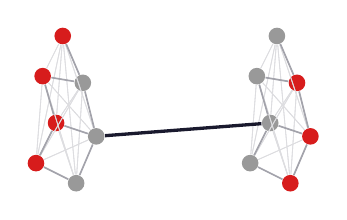
\begin{tikzpicture}[scale=0.85,
            nM/.style={circle, fill=accentred!70!red, minimum size=6pt, inner sep=0pt},
            nG/.style={circle, fill=midgray!60, minimum size=6pt, inner sep=0pt}]
            \node[nM] (L1) at (0,0.3) {};
            \node[nG] (L2) at (0.6,0) {};
            \node[nM] (L3) at (0.3,0.9) {};
            \node[nG] (L4) at (0.9,0.7) {};
            \node[nM] (L5) at (0.1,1.6) {};
            \node[nG] (L6) at (0.7,1.5) {};
            \node[nM] (L7) at (0.4,2.2) {};
            \foreach \i in {L1,L2,L3,L4,L5,L6,L7} {
                \foreach \j in {L1,L2,L3,L4,L5,L6,L7} {
                    \draw[darktext!15, line width=0.3pt] (\i)--(\j);
                }
            }
            \foreach \i/\j in {L1/L2,L2/L4,L3/L4,L3/L5,L5/L6,L6/L7,L1/L3,L4/L6} {
                \draw[darktext!40, line width=0.6pt] (\i)--(\j);
            }
            \node[nG] (R1) at (3.2,0.3) {};
            \node[nM] (R2) at (3.8,0) {};
            \node[nG] (R3) at (3.5,0.9) {};
            \node[nM] (R4) at (4.1,0.7) {};
            \node[nG] (R5) at (3.3,1.6) {};
            \node[nM] (R6) at (3.9,1.5) {};
            \node[nG] (R7) at (3.6,2.2) {};
            \foreach \i in {R1,R2,R3,R4,R5,R6,R7} {
                \foreach \j in {R1,R2,R3,R4,R5,R6,R7} {
                    \draw[darktext!15, line width=0.3pt] (\i)--(\j);
                }
            }
            \foreach \i/\j in {R1/R2,R2/R4,R3/R4,R3/R5,R5/R6,R6/R7,R1/R3,R4/R6} {
                \draw[darktext!40, line width=0.6pt] (\i)--(\j);
            }
            \draw[darktext, line width=1.2pt] (L4)--(R3);
        \end{tikzpicture}
        \end{center}
        \vspace{4pt}
        \resultbox[boxfillred]{accentred}{%
            {\small\color{accentred}\bfseries Small spectral gap}\\[2pt]
            {\small Simplicity delayed---planner must balance resources between competing communities.}
        }
    \end{column}
\end{columns}
\end{frame}

% ============================================================
% SLIDE 8: Golub et al. — Budget & Synthesis Matrix
% ============================================================
\begin{frame}[shrink=8]{Galeotti, Golub, \& Goyal --- Budget and Optimal Targeting}
\accentline
\begin{columns}[T]
    \begin{column}{0.50\textwidth}
        {\color{accentgreen}\bfseries The Planner's Synthesis Matrix}\\[6pt]
        \begin{center}
        \small
        \renewcommand{\arraystretch}{1.5}
        \setlength{\tabcolsep}{5pt}
        \begin{tabular}{
            >{\bfseries}r
            |>{\centering\arraybackslash}p{2.5cm}
            |>{\centering\arraybackslash}p{2.5cm}|}
            \multicolumn{1}{c}{}
            & \multicolumn{1}{c}{\color{accentblue}\bfseries Complements}
            & \multicolumn{1}{c}{\color{accentred}\bfseries Substitutes} \\
            \cline{2-3}
            Small $C$
            & Blend of top PCs. Intervention shaped by status quo. Targets cohesive variables.
            & Blend of bottom PCs. Intervention shaped by status quo. Targets alternating variables. \\
            \cline{2-3}
            Large $C$
            & \textbf{The Simple Intervention.} Pure Eigenvector Centrality ($\mathbf{u}_1$). Global hub targeting.
            & \textbf{The Simple Intervention.} Pure Bipartiteness ($\mathbf{u}_n$). Asymmetric local targeting. \\
            \cline{2-3}
        \end{tabular}
        \end{center}
        \vspace{2pt}
        {\scriptsize\color{midgray} Rows = budget size $C$; columns = sign of $\beta$ (spillover type).}
    \end{column}
    \begin{column}{0.46\textwidth}
        \resultbox[boxfillgreen]{accentgreen}{%
            {\color{accentgreen}\bfseries Budget \& Complexity}\\[3pt]
            {\small \textbf{Low budget} $\to$ intervention is complex: blend of many principal components, heavily shaped by the status quo $\hat{\mathbf{b}}$.\\[3pt]
            \textbf{High budget} $\to$ intervention is simple: snaps to a \textbf{single network statistic}, ignoring the status quo entirely.}
        }
        \vspace{6pt}
        \resultbox[boxfillblue]{accent}{%
            {\color{accent}\bfseries Key Takeaway}\\[3pt]
            {\small With large enough resources, the optimal targeting strategy depends \textbf{only on the network}---not on agents' initial preferences.}
        }
    \end{column}
\end{columns}
\end{frame}

% ============================================================
% SLIDE 9: Morris — Setup
% ============================================================
\begin{frame}[shrink=8]{Morris (2000) --- ``Contagion''}
\accentline
\begin{columns}[T]
    \begin{column}{0.54\textwidth}
        {\small Infinite population on a network. Each pair of neighbors plays a $2 \times 2$ coordination game:}\\[4pt]

        \begin{center}
        {\small
        \begin{tabular}{c|cc}
            & $A$ & $B$ \\\hline
            $A$ & $\color{accentgreen}a, a$ & $b, c$ \\
            $B$ & $c, b$ & $\color{accentred}d, d$ \\
        \end{tabular}}
        \end{center}
        \vspace{2pt}

        \begin{itemize}\small\setlength\itemsep{2pt}
            \item $a > c$, $d > b$: both $(A,A)$ and $(B,B)$ are strict NE
            \item $a > d$: $(A,A)$ {\color{accentgreen}Pareto-dominates}
            \item $a{-}c < d{-}b$: $(B,B)$ {\color{accentred}risk-dominates}
        \end{itemize}
        \vspace{4pt}
        {\small Player switches to $B$ if fraction $\geq q^*$ of neighbors play $B$:}
        \vspace{-4pt}
        \[
            {\color{accentred} q^* = \frac{a - c}{(a-c) + (d-b)}}
        \]
    \end{column}
    \begin{column}{0.42\textwidth}
        \resultbox[boxfill]{accentteal}{%
            {\color{accentteal}\bfseries Key Definitions}\\[4pt]
            {\color{accentgreen}\bfseries Contagious:} {\small $\exists$ a finite set of initial $B$-players such that eventually the \textbf{entire} population plays $B$.}\\[4pt]
            {\color{accentred}\bfseries Uninvadable:} {\small If almost everyone plays $B$, a small group of $A$-players \textbf{cannot} take over.}\\[4pt]
            {\small These are mutually exclusive.}
        }
        \vspace{1pt}
        {\color{accentteal}\bfseries Example}\\[1pt]
        {\small Council members choose to remain honest ($A$) or accept a bribe ($B$). If enough of your political allies switch to $B$, the political risk drops and it becomes worthwhile for you to switch to $B$ too—$B$ spreads contagiously.}
        
    \end{column}
\end{columns}
\end{frame}

% ============================================================
% SLIDE 10: Morris — Contagion on Different Topologies
% ============================================================
\begin{frame}[shrink=15]{Morris --- Contagion on Different Topologies}
\accentline
\begin{columns}[T]
    \begin{column}{0.50\textwidth}
        {\color{accentteal}\bfseries The Geometry Breakdown}\\[4pt]
        {\small Different network topologies yield different contagion thresholds:}\\[6pt]
        \begin{center}
        \small
        \renewcommand{\arraystretch}{1.4}
        \begin{tabular}{l c c}
            \toprule
            \textbf{Topology} & \textbf{Max degree} & \textbf{Threshold $\xi$} \\
            \midrule
            Line & $2$ & $1/2$ \\
            $m$-dim.\ Lattice & $2m$ & $1/2m$ \\
            Regions & $m{+}1$ & $1/(m{+}1)$ \\
            Hierarchy & $m{+}1$ & $1/(m{+}1)$ \\
            \bottomrule
        \end{tabular}
        \end{center}
        \vspace{6pt}
        {\color{accentteal}\bfseries Example: Line vs.\ Grid}\\[3pt]
        \begin{center}
        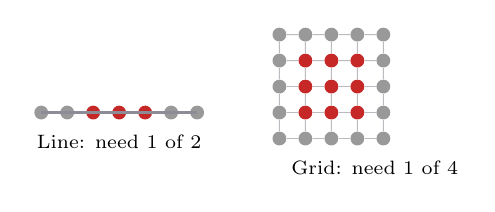
\begin{tikzpicture}[scale=0.55,
            nd/.style={circle, fill=lightgray, minimum size=5pt, inner sep=0pt},
            hot/.style={circle, fill=accentred, minimum size=5pt, inner sep=0pt}]
            % Line
            \node[nd] at (0,0) {};
            \node[nd] at (0.6,0) {};
            \node[hot] at (1.2,0) {};
            \node[hot] at (1.8,0) {};
            \node[hot] at (2.4,0) {};
            \node[nd] at (3.0,0) {};
            \node[nd] at (3.6,0) {};
            \draw[darktext!50, thick] (0,0)--(0.6,0)--(1.2,0)--(1.8,0)--(2.4,0)--(3.0,0)--(3.6,0);
            \node[below, font=\scriptsize] at (1.8,-0.3) {Line: need 1 of 2};
            % Grid
            \foreach \x in {0,...,4} {
                \foreach \y in {0,...,4} {
                    \pgfmathparse{(\x>=1 && \x<=3 && \y>=1 && \y<=3) ? 1 : 0}
                    \ifnum\pgfmathresult=1
                        \node[hot] (g\x\y) at (5.5+\x*0.6, \y*0.6-0.6) {};
                    \else
                        \node[nd] (g\x\y) at (5.5+\x*0.6, \y*0.6-0.6) {};
                    \fi
                }
            }
            \foreach \x in {0,...,4} {
                \foreach \y [evaluate=\y as \ny using int(\y+1)] in {0,...,3} {
                    \draw[darktext!30, thin] (g\x\y)--(g\x\ny);
                }
            }
            \foreach \y in {0,...,4} {
                \foreach \x [evaluate=\x as \nx using int(\x+1)] in {0,...,3} {
                    \draw[darktext!30, thin] (g\x\y)--(g\nx\y);
                }
            }
            \node[below, font=\scriptsize] at (7.7,-0.9) {Grid: need 1 of 4};
        \end{tikzpicture}
        \end{center}
    \end{column}
    \begin{column}{0.46\textwidth}
        \resultbox[boxfillred]{accentred}{%
            {\color{accentred}\bfseries Takeaway 1}\\[3pt]
            {\small More connections $\neq$ easier spread. In deterministic best-response games, higher-dimensional networks require \textbf{more converted neighbors} in absolute terms to reach proportion $q^*$.\\[2pt]
            A line needs 1 of 2; a grid needs 1 of 4.}
        }
        \vspace{6pt}
        \resultbox[boxfillblue]{accent}{%
            {\color{accent}\bfseries Takeaway 2}\\[3pt]
            {\small Specific geometric lattices yield \textbf{inconsistent, structure-dependent} thresholds. To build a universal theory of contagion, Morris abandons shape and looks for \textbf{deeper properties}---cohesion.}
        }
    \end{column}
\end{columns}
\end{frame}

% ============================================================
% SLIDE 11: Morris — Cohesion, Weak Ties, and the Upper Bound
% ============================================================
\begin{frame}[shrink=8]{Morris --- Cohesion and the Limits of Contagion}
\accentline
\begin{columns}[T]
    \begin{column}{0.52\textwidth}
        {\color{accentteal}\bfseries $p$-Cohesion}\\[3pt]
        {\small A group is \textbf{$p$-cohesive} if every member has at least proportion $p$ of their interactions strictly within the group.}\\[4pt]
        {\small Contagion stops instantly when it hits a group that is too inward-looking. If a group's internal ties are stronger than the external pressure, the behavior \textbf{cannot penetrate}.}\\[8pt]

        {\color{accentteal}\bfseries Proposition 1 (Upper Bound)}\\[3pt]
        \begin{center}
        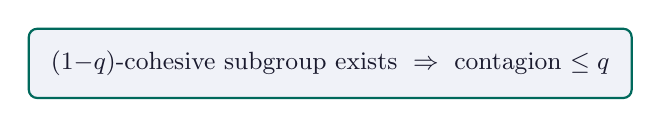
\begin{tikzpicture}
            \node[fill=boxfill, draw=accentteal, rounded corners=3pt, line width=0.8pt, inner sep=8pt, text=darktext, font=\small] {
                $(1{-}q)$-cohesive subgroup exists $\;\Rightarrow\;$ contagion $\leq q$
            };
        \end{tikzpicture}
        \end{center}
        \vspace{2pt}
        {\small The contagion threshold $\xi$ is perfectly bounded by the smallest internal cohesion that can form an infinite roadblock.\\[2pt]
        \color{midgray}\textit{Translation:} you can only spread a behavior if the network's most insular clique can be breached by $q^*$.}
    \end{column}
    \begin{column}{0.44\textwidth}
        \resultbox[boxfillgreen]{accentgreen}{%
            {\color{accentgreen}\bfseries Spreading Information}\\
            {\small(Weak Ties --- Granovetter)}\\[3pt]
            {\small Hearing a rumor \textbf{once} is enough. Thrives on high neighbor growth. Relies on long-range, non-overlapping connections.}
        }
        \vspace{4pt}
        \resultbox[boxfillred]{accentred}{%
            {\color{accentred}\bfseries Changing a Convention}\\
            {\small(Strong Ties --- Morris)}\\[3pt]
            {\small Requires \textbf{local critical mass} to cross threshold $q^*$. Thrives on low neighbor growth. Needs strong, overlapping local ties.}
        }
    \end{column}
\end{columns}
\end{frame}

% ============================================================
% SLIDE 12: Connecting the Papers — Our Model
% ============================================================
\begin{frame}[shrink=8]{Connecting the Papers: Our Model}
\accentline
\vspace{-4pt}
\begin{center}
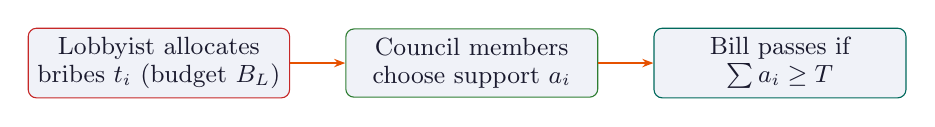
\begin{tikzpicture}[
    box/.style={fill=boxfill, rounded corners=3pt, text=darktext, font=\small, minimum width=3.2cm, minimum height=0.65cm, align=center},
    arr/.style={-{Stealth[length=4pt]}, thick, accentorange}
]
    \node[box, draw=accentred] (s1) {Lobbyist allocates\\[-1pt]bribes $t_i$ (budget $B_L$)};
    \node[box, draw=accentgreen, right=0.7cm of s1] (s2) {Council members\\[-1pt]choose support $a_i$};
    \node[box, draw=accentteal, right=0.7cm of s2] (s3) {Bill passes if\\[-1pt]$\sum a_i \geq T$};
    \draw[arr] (s1) -- (s2);
    \draw[arr] (s2) -- (s3);
\end{tikzpicture}
\end{center}
\vspace{-2pt}
{\small\color{accentgreen}\bfseries Payoff:}
\vspace{-6pt}
\[
    \boxed{U_i = a_i\!\left(\underbrace{{\color{accentred}b_i + t_i}}_{\text{\tiny Shleifer \& Vishny}} + \underbrace{{\color{accentgreen}\beta \sum_j g_{ij} a_j}}_{\text{\tiny Golub et al.}}\right) - \tfrac{1}{2}\,c\,a_i^2}
\]
\vspace{-12pt}
\begin{columns}[T]
    \begin{column}{0.50\textwidth}
        \begin{itemize}\small\setlength\itemsep{2pt}
            \item {\color{accentred}$b_i + t_i$}: baseline inclination + lobbyist's bribe
            \item {\color{accentgreen}$\beta \sum g_{ij}a_j$}: peer effects---cost of supporting the bill drops when friends also support it
            \item {\color{accentteal}Contagion}: does support spread from one bribed member through the network?
        \end{itemize}
    \end{column}
    \begin{column}{0.46\textwidth}
        \resultbox[boxfillorange]{accentorange}{%
            {\color{accentorange}\bfseries Note}\\[3pt]
            {\small In Golub et al., the planner is \textbf{benevolent} (maximizes welfare). In our model, the lobbyist is \textbf{adversarial} (maximizes corruption).\\[2pt]}
        }
    \end{column}
\end{columns}
\end{frame}

% ============================================================
% SLIDE 13: Research Questions
% ============================================================
\begin{frame}{3 Questions}
\accentline
\vspace{4pt}

\resultbox[boxfillgreen]{accentgreen}{%
    {\color{accentgreen}\bfseries Q1}\quad
    {\small\bfseries How does the network structure of a council affect the lobbyist's optimal bribery strategy and the equilibrium level of support?}\\[3pt]
    {\scriptsize\color{midgray} $\to$ Connects to Golub et al.: eigenvector centrality, principal components, spectral gap}
}

\vspace{8pt}

\resultbox[boxfillblue]{accentblue}{%
    {\color{accentblue}\bfseries Q2}\quad
    {\small\bfseries Under what conditions does bribing one council member cause support to spread contagiously through the network?}\\[3pt]
    {\scriptsize\color{midgray} $\to$ Connects to Morris: contagion thresholds, network topology, $q^*$ condition}
}

\vspace{8pt}

\resultbox[boxfillorange]{accentorange}{%
    {\color{accentorange}\bfseries Q3}\quad
    {\small\bfseries What voting rule (majority, supermajority, weighted) is most robust to outside lobbying, given the council's network structure?}\\[3pt]
    {\scriptsize\color{midgray} $\to$ Novel design question: which threshold $T$ minimizes the lobbyist's ability to pass the bill?}
}
\end{frame}

% ============================================================
% SLIDE 14: References
% ============================================================
\begin{frame}[plain]
    \vspace{2cm}
    \begin{center}
        {\color{accent}\rule{0.35\textwidth}{1.5pt}}\\[10pt]
        {\LARGE\bfseries\color{darktext} Thank You}\\[4pt]
        {\small\color{midgray}
        \textbf{References:}\\[8pt]
        Shleifer, A.\ and Vishny, R.W.\ (1993).
        ``Corruption.'' \textit{Quarterly Journal of Economics}, 108(3), 599--617.\\[6pt]
        Galeotti, A., Golub, B., and Goyal, S.\ (2020).
        ``Targeting Interventions in Networks.'' \textit{Econometrica}, 88(6), 2445--2471.\\[6pt]
        Morris, S.\ (2000).
        ``Contagion.'' \textit{Review of Economic Studies}, 67(1), 57--78.
        }
    \end{center}
\end{frame}

\end{document}

